%Jennifer Pan, August 2011

\documentclass[10pt,letter]{article}
	% basic article document class
	% use percent signs to make comments to yourself -- they will not show up.

\usepackage{amsmath}
\usepackage{amssymb}
\usepackage{tikz}
	% packages that allow mathematical formatting

\usepackage{graphicx}
	% package that allows you to include graphics

\usepackage{setspace}
	% package that allows you to change spacing

\onehalfspacing
	% text become 1.5 spaced

\usepackage{fullpage}
	% package that specifies normal margins

\renewcommand{\vector}[1]{\boldsymbol{#1}}
\newcommand{\problem}[1]{\section*{Problem #1}}
\newcommand{\problempart}[1]{\paragraph{#1}}

\begin{document}
	% line of code telling latex that your document is beginning


\title{Problem Set 2}

\author{Nicholas Wu}

\date{Fall 2020}
	% Note: when you omit this command, the current dateis automatically included

\maketitle
	% tells latex to follow your header (e.g., title, author) commands.
\textbf{Note:} I use bold symbols to denote vectors and nonbolded symbols to denote scalars. I primarily use vector notation to shorthand some of the sums, since many of the sums are dot products.

\problem{1}

\problempart{(1)} The Bellman equation is given by
\[ V(k, z) = \max_{h, k'} \left(u(c, 1-h) + \beta \sum_{z'} \pi(z' | z) V(k', z')\right) \]
subject to
\[ c + k' \le f(k, z, h) + (1-\delta)k \]
\problempart{(2)}
Taking FOCs, we find:
\[ u_1(c, 1-h) = \beta \sum_{z'} \pi(z' | z) V_1(k', z') \]
\[ -u_2(c, 1-h) + u_1(c, 1-h) f_3(k, z, h) z = 0 \]
The envelope theorem gives
\[ V_1(k, z) = u_1(c, 1-h) \left(1 - \delta + f_1(k, z, h)\right) \]
so we can rewrite the first FOC as
\[ u_1(c, 1-h) = \beta \sum_{z'} \pi(z' | z) u_1(c', 1-h') \left(1 - \delta + f_1(k', z', h')\right) \]
\problempart{(3)}
No. The FOC determining labor is
\[ -u_2(c, 1-h) + u_1(c, 1-h) f_3(k, z, h) = 0 \]
and is fully categorized by the current state and capital levels. Hence there is no state uncertainty in determining labor supply.
\problempart{(4)}
We guess that the labor law of motion is constant for some $h^*$ and the capital supply follows the functional form:
\[ k' = Czk^\alpha h^{1-\alpha} \]
then
\[ c = zk^\alpha h^{1-\alpha}(1-C) \]
The Euler equation gives
\[ 1/c = \beta \sum_{z'} \pi(z' | z)  \frac{ \alpha z' (k')^{\alpha - 1}(h')^{1-\alpha}}{(1-C)z' (k')^\alpha (h')^{1-\alpha}} \]
\[ \frac{1}{zk^\alpha h^{1-\alpha}} = \beta  \frac{ \alpha }{k'} \]
\[ \frac{1}{zk^\alpha h^{1-\alpha}} = \beta  \frac{ \alpha }{Czk^\alpha h^{1-\alpha}} \]
\[C  = \beta\alpha \]
So capital evolves as
\[ k' = \alpha\beta zk^\alpha h^{1-\alpha} \]
The labor condition is
\[ \gamma g'(h) = \frac{1}{c} (1-\alpha)zk^\alpha h^{-\alpha}  \]
\[ \gamma g'(h) = \frac{1}{zk^\alpha h^{-\alpha}(1-\alpha\beta)} (1-\alpha)zk^\alpha h^{1-\alpha}  \]
\[ \gamma g'(h) = \frac{1}{zk^\alpha h^{-\alpha}(1-\alpha\beta)} (1-\alpha)zk^\alpha h^{1-\alpha}  \]
\[ h^* g'(h^*) = \frac{1-\alpha}{\gamma(1-\alpha\beta)} \]
which should pin down $h^*$.
\problempart{(5)}
There is no labor supply fluctuation; in this model, labor is constant. The change in wages as a result of increases/decreases in technology does not affect the amount of labor supplied.
\pagebreak

\problem{2}
\problempart{(1)} The Bellman equations are
\[ V_H(k) = \max_{k'}\left[ u(z_H k^\alpha + (1-\delta) k - k') + \beta \pi_{HH}V_H(k')+ \beta \pi_{HL}V_L(k') \right] \]
\[ V_L(k) = \max_{k'}\left[ u(z_L k^\alpha + (1-\delta) k - k') + \beta \pi_{LH}V_H(k')+ \beta \pi_{LL}V_L(k') \right] \]
\problempart{(2)} We guess
\[ V_H(k) = a_H + b_H \log k \]
\[ V_L(k) = a_L + b_L \log k \]
Pluggin into the Bellman equations:
\[ a_H + b_H \log k = \max_{k'}\left[ \log(z_H k^\alpha + (1-\delta) k - k') + \beta \pi_{HH}(a_H + b_H \log k')+ \beta \pi_{HL}(a_L + b_L \log k') \right] \]
\[ a_L + b_L \log k = \max_{k'}\left[ \log(z_L k^\alpha + (1-\delta) k - k') + \beta \pi_{LH}(a_H + b_H \log k')+ \beta \pi_{LL}(a_L + b_L \log k') \right] \]
Taking the maximiation FOC of the first:
\[ \frac{1}{z_H k^\alpha + (1-\delta) k - k'} = \beta \pi_{HH} b_H \frac{1}{k'} + \beta \pi_{HL} b_L\frac{1}{k'}\]
\[ \frac{k'}{z_H k^\alpha + (1-\delta) k - k'} = \beta (\pi_{HH} b_H + \pi_{HL} b_L)\]
\[ k' = \beta (\pi_{HH} b_H + \pi_{HL} b_L)(z_H k^\alpha + (1-\delta) k - k')\]
\[ k'(1 + \beta (\pi_{HH} b_H + \pi_{HL} b_L)) = \beta (\pi_{HH} b_H + \pi_{HL} b_L)(z_H k^\alpha + (1-\delta) k )\]
\[ k' = \frac{\beta (\pi_{HH} b_H + \pi_{HL} b_L)(z_H k^\alpha + (1-\delta) k )}{1 + \beta (\pi_{HH} b_H + \pi_{HL} b_L)}\]
Plugging into the first FOC, using $\delta = 1$, and isolating only the $k$ terms, we get
\[ b_H \log k = \alpha \log k + \alpha \beta(\pi_{HH}b_H+ \pi_{HL}b_L) \log k \]
\[ b_H = \alpha( 1 + \beta(\pi_{HH}b_H+ \pi_{HL}b_L) ) \]
Doing the same the second FOC, we get
\[ b_L = \alpha( 1 + \beta(\pi_{LH}b_H + \pi_{LL}b_L)) \]
Solving, we get
\[ b_L = b_H = \frac{\alpha}{1 - \alpha \beta} \]
We can also solve for $a_H, a_L$, but we can determine the optimal policies and the path of capital from just $b$.
The optimal policies are
\[ k'_H = \frac{\beta b_H z_H k^\alpha }{1 + \beta b_H} = \alpha \beta z_H k^\alpha \]
\[ k'_L = \frac{\beta b_L z_L k^\alpha }{1 + \beta b_L}= \alpha \beta z_L k^\alpha \]
\problempart{(3)} If the state is always $z_L$, then capital just converges to the steady state at $z_L$, which is
\[ k^*_L = (\alpha \beta z_L)^{1/(1-\alpha)} \]
\problempart{(4)} We recall from our observation from the last problem set that $\log$ utility is the limit case of the CRRA as $\theta = 1$, and the income/substitution effects balance out, and the savings rate is constant. We thus note then that changing $\pi_{HH}$ and $\pi_{LL}$ has no effect on the law of motion of capital.
\pagebreak
\problem{3}
\problempart{(1)}
See figure 1.
The IES is
\[ \frac{1}{\epsilon_u} = -\frac{u'(c)}{u''(c)c} = \frac{c^{-\theta}}{\theta c^{-\theta}} = \frac{1}{\theta} \]
Using the Euler equation from lecture, we get
\[ \frac{\dot{c}(t) }{c(t)} = \frac{f'(k(t)) - \delta - \rho}{\theta} \]
and the TVC is
\[ \lim_{t \to \infty} \left[ e^{-\rho t} c(t)^{-\theta} k(t) \right] \]
Finally, the budget constraint yields
\[ \dot{k}(t) = f(k(t)) - \delta k(t) - c(t) \]
\begin{figure}
\begin{centering}
\begin{tikzpicture}
\draw[thick,->] (0,0) -- (8,0) node[anchor=north west] {$k$};
\draw[thick,->] (0,0) -- (0,6) node[anchor=south east] {$c$};
\draw[red] (3,6) -- (3,0) node[anchor=north] {$\dot{c} = 0$};
\draw[red] (0,0) .. controls (2,4) and (5,4) .. (6,0) node[anchor=north] {$\dot{k} = 0$};
\draw[red, thick] (1,0.5) .. controls (2,1) .. (3,3) node[anchor=north west] {Stable arm};
\draw[red, thick] (5,5.5) .. controls (4,5) .. (3,3);
\end{tikzpicture}
\caption{Phase diagram, part 1}
\end{centering}
\end{figure}
\problempart{(2)}
See figure 2 for the change in the phase diagram. If the IES is larger than 1, the new saddle path will be below the old steady state, since consumers are more willing to give up their current consumption to increase the capital stock for future consumption. If the IES is less than 1, the new saddle path will be above the old steady state, since consumers will invest a smaller fraction of their income and get to the new steady state slower.
\begin{figure}
\begin{centering}
\begin{tikzpicture}
\draw[thick,->] (0,0) -- (10,0) node[anchor=north west] {$k$};
\draw[thick,->] (0,0) -- (0,10) node[anchor=south east] {$c$};
\draw[red] (2.75,10) -- (2.75,0) node[anchor=north] {$\dot{c} = 0$};
\draw[red] (0,0) .. controls (2,4) and (4.5,4) .. (5,0) node[anchor=south east] {$\dot{k} = 0$};
\draw[blue] (5.5,10) -- (5.5,0) node[anchor=north] {$\dot{c} = 0$};
\draw[blue] (0,0) .. controls (4,8) and (9,8) .. (10,0) node[anchor=south east] {$\dot{k} = 0$};
\draw[brown] (5.5, 5.9) -- (2.75, 3.3)  node[anchor = south east] {$\theta > 1$};
\draw[purple] (5.5, 5.9) -- (2.75, 1.7)  node[anchor = south east] {$\theta < 1$};
\end{tikzpicture}
\caption{Phase diagram, part 2. Red is the old state, blue the new state}
\end{centering}
\end{figure}
\problempart{(3)}
Assuming the functional form from part (2), the characteristic conditions are
\[ \frac{\dot{c}(t) }{c(t)} = \frac{Af'(k(t)) - \delta - \rho}{\theta} \]
\[ \dot{k}(t) = Af(k(t)) - \delta k(t) - c(t) \]
\[ \lim_{t \to \infty} \left[ e^{-\rho t} c(t)^{-\theta} k(t) \right] \]
At steady state, the desired quantities are determined by:
\[ Af'(k^*) = \delta + \rho\]
\[ c^* = Af(k^*) - \delta k^*\]
\[ i^* = \delta k^* \]
\[ r^* = \rho \]
\[ w^* = c^* - r^* k^* \]
We plot the relevant qualitative paths in figures 3-6. We note that $r$ remains unchanged, and hence is just a straight horizontal line, so we omit this graph. We also note that the investment path depends on the magnitude of $\delta$, and its shape is harder to draw without understanding how large $\delta k(t)$ is relative to $\dot{k}(t)$.
\begin{figure}
\begin{centering}
\begin{tikzpicture}
\draw[thick,->] (0,0) -- (8,0) node[anchor=north west] {$t$};
\draw[thick,->] (0,0) -- (0,4) node[anchor=south east] {$k$};
\draw[dashed] (0,1) -- (8,1) node[anchor=west] {old steady state};
\draw[dashed] (0,3) -- (8,3) node[anchor=west] {new steady state};
\draw (0,1) .. controls (0.5,2) and (1,3) .. (8,3);
\end{tikzpicture}
\caption{Path of capital after shock}
\end{centering}
\end{figure}
\begin{figure}
\begin{centering}
\begin{tikzpicture}
\draw[thick,->] (0,0) -- (8,0) node[anchor=north west] {$t$};
\draw[thick,->] (0,0) -- (0,4) node[anchor=south east] {$c$};
\draw[dashed] (0,1) -- (8,1) node[anchor=west] {old steady state};
\draw[dashed] (0,3) -- (8,3) node[anchor=west] {new steady state};
\draw (0,1.5) .. controls (0.5,2.5) and (1,3) .. (8,3);
\end{tikzpicture}
\caption{Path of consumption after shock}
\end{centering}
\end{figure}
\begin{figure}
\begin{centering}
\begin{tikzpicture}
\draw[thick,->] (0,0) -- (8,0) node[anchor=north west] {$t$};
\draw[thick,->] (0,0) -- (0,4) node[anchor=south east] {$y$};
\draw[dashed] (0,1) -- (8,1) node[anchor=west] {old steady state};
\draw[dashed] (0,3) -- (8,3) node[anchor=west] {new steady state};
\draw (0,1.5) .. controls (0.5,2) and (1,3) .. (8,3);
\end{tikzpicture}
\caption{Path of output after shock.}
\end{centering}
\end{figure}
\begin{figure}
\begin{centering}
\begin{tikzpicture}
\draw[thick,->] (0,0) -- (8,0) node[anchor=north west] {$t$};
\draw[thick,->] (0,0) -- (0,4) node[anchor=south east] {$w$};
\draw[dashed] (0,1) -- (8,1) node[anchor=west] {old steady state};
\draw[dashed] (0,3) -- (8,3) node[anchor=west] {new steady state};
\draw (0,1.5) .. controls (0.5,2) and (1,3) .. (8,3);
\end{tikzpicture}
\caption{Path of wages after shock.}
\end{centering}
\end{figure}
\problempart{(4)} In the previous part, we characterized the responses to a sudden impulse shock to the economy (in the total factor productivity).
\pagebreak
\problem{4}
\problempart{(1)}
The present value Hamiltonian is
\[ H(a, c, \mu) = \frac{c(t)^{1-\theta} - 1}{1-\theta} + \mu(t)\left( (1-\tau(t))r(t)a(t) + w(t) - c(t) + T(t) \right) \]
The optimization conditions are given by
\[ c(t)^{-\theta} = \mu(t) \]
\[ (1-\tau(t))r(t)\mu(t) = - \dot{\mu}(t) + \rho \mu(t)  \]
\[ \dot{a}(t) = (1-\tau(t))r(t)a(t) + w(t) - c(t) + T(t) \]
\[ \lim_{t \to \infty} e^{-\rho t}\mu(t)a(t) = 0 \]
Combining the first two, we get
\[ (1-\tau(t))r(t) -\rho = -\dot{\mu}(t) /\mu(t)  \]
\[ \frac{(1-\tau(t))r(t) - \rho}{\theta} = \dot{c}(t) /c(t)  \]
Using the firm maximizing rates and wages,
\[ r(t) = f'(k(t)) - \delta \]
\[ w(t) = f(k(t)) - k(t) f'(k(t)) \]
We can rewrite our conditions as
\[  \frac{\dot{c}(t)} {c(t)}  = \frac{(1-\tau(t))(f'(k(t)) - \delta) - \rho}{\theta}  \]
\[ \lim_{t \to \infty} e^{-\rho t}c(t)^{-\theta} k(t) = 0 \]
and
\[ \dot{k}(t) = (1-\tau(t))(f'(k(t)) - \delta)k(t) + f(k(t)) - k(t) f'(k(t)) - c(t) + T(t) \]
\[ \dot{k}(t) = (1-\tau(t))(f'(k(t)) - \delta)k(t) + f(k(t)) - k(t) f'(k(t)) - c(t) + \tau(t)(f'(k(t)) - \delta)k(t) \]
\[ \dot{k}(t) =  f(k(t)) - \delta k(t)  - c(t)  \]

\problempart{(2)} See figure 7.
\begin{figure}
\begin{centering}
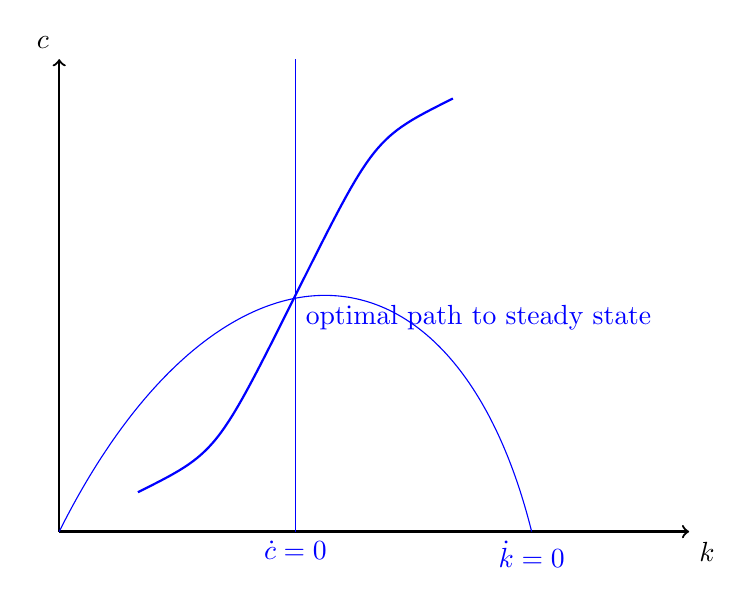
\begin{tikzpicture}
\draw[thick,->] (0,0) -- (8,0) node[anchor=north west] {$k$};
\draw[thick,->] (0,0) -- (0,6) node[anchor=south east] {$c$};
\draw[blue] (3,6) -- (3,0) node[anchor=north] {$\dot{c} = 0$};
\draw[blue] (0,0) .. controls (2,4) and (5,4) .. (6,0) node[anchor=north] {$\dot{k} = 0$};
\draw[blue, thick] (1,0.5) .. controls (2,1) .. (3,3) node[anchor=north west] {optimal path to steady state};
\draw[blue, thick] (5,5.5) .. controls (4,5) .. (3,3);
\end{tikzpicture}
\caption{Phase diagram, part 2}
\end{centering}
\end{figure}
\problempart{(3)} See figure 8. Consumption will increase in order to converge to the new steady state.
\begin{figure}
\begin{centering}
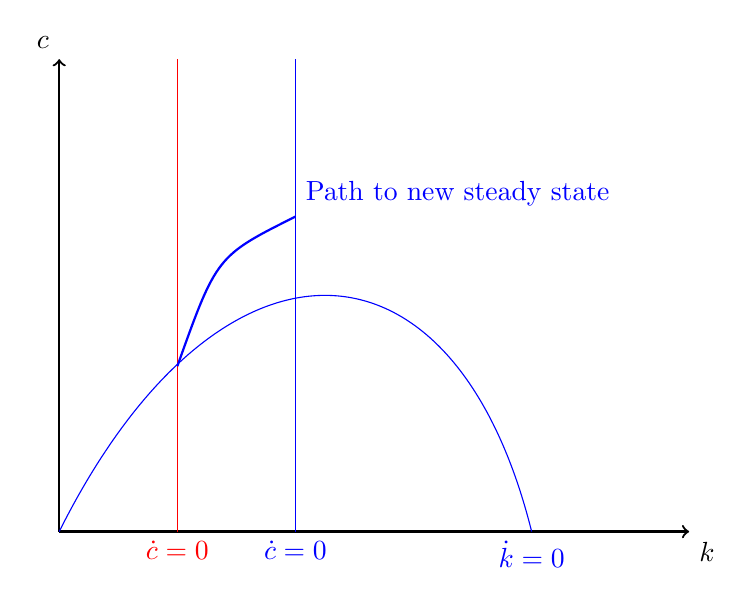
\begin{tikzpicture}
\draw[thick,->] (0,0) -- (8,0) node[anchor=north west] {$k$};
\draw[thick,->] (0,0) -- (0,6) node[anchor=south east] {$c$};
\draw[blue] (3,6) -- (3,0) node[anchor=north] {$\dot{c} = 0$};
\draw[red] (1.5,6) -- (1.5,0) node[anchor=north] {$\dot{c} = 0$};
\draw[blue] (0,0) .. controls (2,4) and (5,4) .. (6,0) node[anchor=north] {$\dot{k} = 0$};
\draw[blue, thick] (1.5,2.1) .. controls (2,3.5) .. (3,4) node[anchor=south west] {Path to new steady state};
\end{tikzpicture}
\caption{Phase diagram, part 3}
\end{centering}
\end{figure}
\problempart{(4)} See figure 9. The consumers will begin decreasing capital and increasing consumption in anticipation of the policy change.
\begin{figure}
\begin{centering}
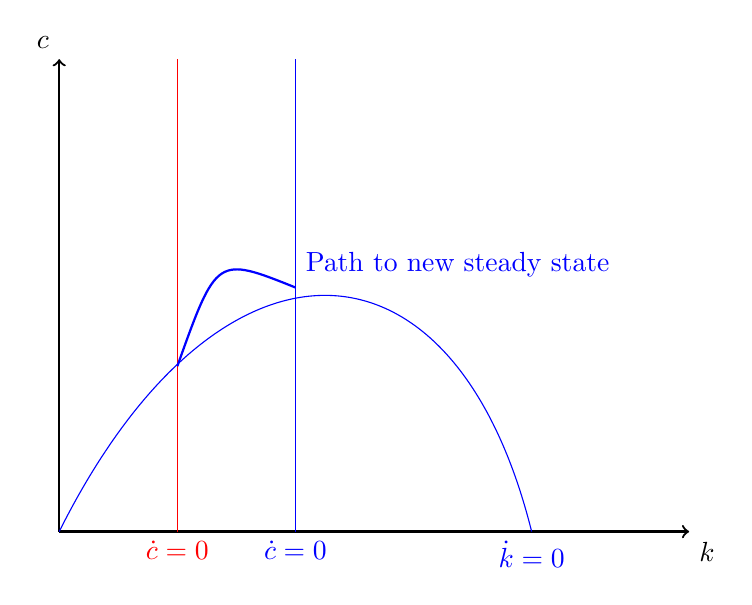
\begin{tikzpicture}
\draw[thick,->] (0,0) -- (8,0) node[anchor=north west] {$k$};
\draw[thick,->] (0,0) -- (0,6) node[anchor=south east] {$c$};
\draw[blue] (3,6) -- (3,0) node[anchor=north] {$\dot{c} = 0$};
\draw[red] (1.5,6) -- (1.5,0) node[anchor=north] {$\dot{c} = 0$};
\draw[blue] (0,0) .. controls (2,4) and (5,4) .. (6,0) node[anchor=north] {$\dot{k} = 0$};
\draw[blue, thick] (1.5,2.1) .. controls (2,3.5) .. (3,3.1) node[anchor=south west] {Path to new steady state};
\end{tikzpicture}
\caption{Phase diagram, part 3}
\end{centering}
\end{figure}
\problempart{(5)} See figure 10. The consumers will begin decreasing capital and increasing consumption in anticipation of the policy change, but as soon as the policy change does not come, they will drop consumption to return to the original steady state.
\begin{figure}
\begin{centering}
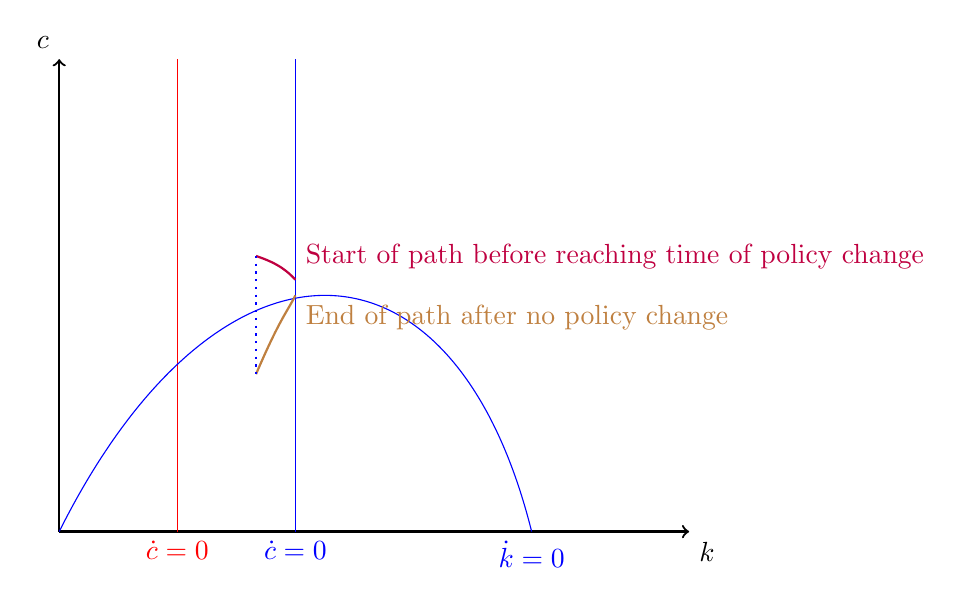
\begin{tikzpicture}
\draw[thick,->] (0,0) -- (8,0) node[anchor=north west] {$k$};
\draw[thick,->] (0,0) -- (0,6) node[anchor=south east] {$c$};
\draw[blue] (3,6) -- (3,0) node[anchor=north] {$\dot{c} = 0$};
\draw[red] (1.5,6) -- (1.5,0) node[anchor=north] {$\dot{c} = 0$};
\draw[blue] (0,0) .. controls (2,4) and (5,4) .. (6,0) node[anchor=north] {$\dot{k} = 0$};
\draw[purple, thick] (2.5,3.5) .. controls (2.8, 3.4) and (2.9, 3.3) .. (3,3.2) node[anchor=south west] {Start of path before reaching time of policy change};
\draw[brown, thick] (2.5,2) .. controls (2.8, 2.7) and (2.9, 2.8) .. (3,3) node[anchor=north west] {End of path after no policy change};
\draw[blue, thick, dotted] (2.5, 3.5) -- (2.5, 2);
\end{tikzpicture}
\caption{Phase diagram, part 3}
\end{centering}
\end{figure}
\end{document}
	% line of code telling latex that your document is ending. If you leave this out, you'll get an error
